\documentclass[10pt,a4paper, twocolumn]{article}
\usepackage[latin1]{inputenc}

% layout
\setlength{\columnsep}{0.75cm}
\usepackage[margin=2.0cm]{geometry}

%\usepackage{url}
%\usepackage{booktabs}

\usepackage{amsmath}
\usepackage{amsfonts}
\usepackage{amssymb}
\usepackage{subfigure}
\usepackage{graphicx}
\usepackage{nonfloat}
\graphicspath{{imgs/}}

\usepackage{xspace}
\newcommand*{\eg}{e.g.\@\xspace}
\newcommand*{\ie}{i.e.\@\xspace}
\newcommand*{\ea}{et al.\@\xspace}
%\renewcommand{\arraystretch}{1.5}

\newcommand{\prob}{Pr}
\newcommand{\rgbdimage}{\mathbf{I}}
\newcommand{\imregion}{\mathcal{R}}
\newcommand{\occ}{o}
\newcommand{\basisshape}{B}
\newcommand{\pcloud}{\mathcal{P}}
\newcommand{\point}{\mathbf{p}}
\newcommand{\normal}{\mathbf{n}}

\title{Predicting Voxel Occupancy From a Single RGBD Image}

\author{Michael Firman}

\begin{document}
\maketitle

\abstract{
	Gaining a representation of the geometry of a scene is an essential task for many applications including robotic navigation, scene re-lighting and object manipulation. 
	Most existing works to recover the scene geometry rely on combining multiple views of the scene captured from many different directions or use of \emph{a priori} information about the expected semantic make-up of the scene.

	We present a method to predict whether or not each voxel in a scene is occupied given just a single RGBD image.
	We argue that objects of dissimilar semantic classes often share similar shapes; this allows for a limited dataset of CAD objects to model the shape of a wide range of objects and hence estimate the hidden geometry of arbitrary scenes.

	Our method comprises of three main stages. 
	First, we propose CAD models which match regions in our input scene, and estimate a suitable transformation into the scene. 
	Next we classify each proposal as being `good' or `bad', using a random forest trained on scenes with known geometry.
	Finally we combine the voxel predictions of all the proposals, taking into account the output of the per-proposal classifier.
}

\begin{figure*}
	\centering% 
	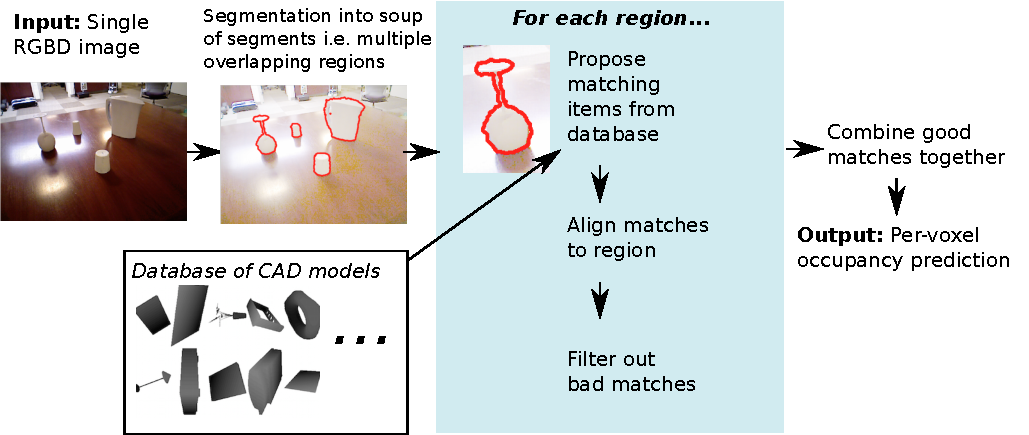
\includegraphics[width=0.9\linewidth]{pipeline_hor}% 
	\figcaption{The pipeline --- a work in progress! This will ultimately show a much more challenging image, together with the basis shapes that are matched in and a visualisation of the final voxel occupancy.}% 
	\label{fig:input.eps}% 
\end{figure*}

%\begin{minipage}{\linewidth} 
%\begin{figure*}[b]
%       \centering 
%       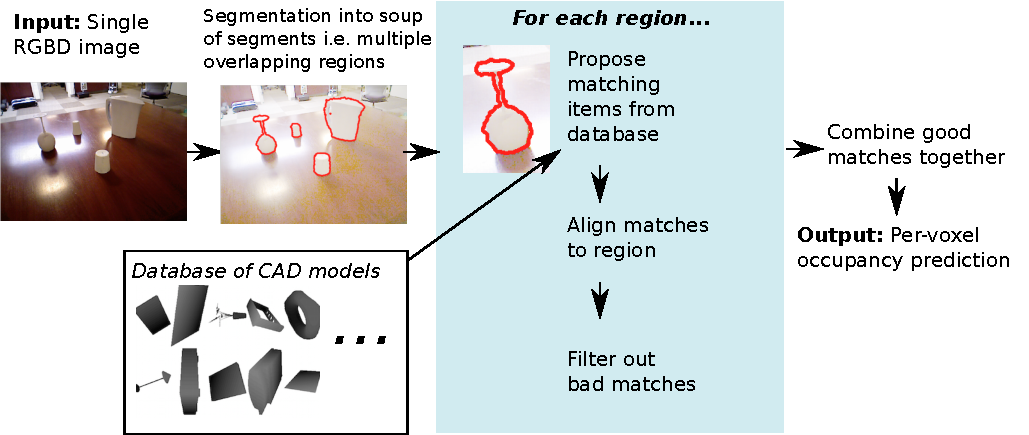
\includegraphics[width=0.6\columnwidth]{pipeline_hor}
%       \caption{The pipeline used --- work in progress!}
%       \label{fig:pipeline}
%\end{figure*}

%\begin{multicols}{2}

\section{Introduction}
Given a single image of a scene, humans can usually get a good overview of the scene and what the geometry is, even in the many areas which are not directly observable. 
We are able to do this using a manner of different tools at our disposal. 
We can use symmetry, hypothesising that unobserved regions match the parts we can see under a transform.
In many occasions we exploit semantic knowledge: by recognising specific objects and relating them to objects in our memory, we form an idea of their shape.
In many cases, however, we use a more generic, higher level knowledge about shape in order to hypothesise the missing regions.

%However, a single image only sees a small subset of the actual visible surfaces in the scene, and can only directly infer a very small number of occupied voxels.


\paragraph{Motivation}
It can be very useful for a computer system to know the geometry of hidden areas of a scene, for reasons such as:

\begin{itemize}
\item \textbf{Robotics} --- Helping a robot to plan a path around objects given only a single view of a scene, e.g. from a doorway. Also to help a robot plan grasping position on objects it can only see partial views of.
\item \textbf{Scene relighting} --- Enabling realistic-looking shadows to be cast from a light moved to a new position in the image.
\item \textbf{Object repositioning} --- Interactive repositioning of objects in the scene. Knowing the voxel occupancy allows a constraint to be placed on where objects can be moved to. (\eg Zheng \ea, Interactive images)
\item \textbf{Re-rendering scene from a new viewpoint}
\end{itemize}

\paragraph{Aim of the system and overview}
Given a single RGBD image, the aim of our system is to predict whether each voxel in the scene is occupied or not - in effect, we want to predict the voxelised occupancy grid of KinectFusion \cite{izadi-uist-2011}, but having been given only a single view of the scene instead of multiple views.

We [plan to] achieve this by matching regions from the input image to renders of objects in a training database.
The voxel occupancy of these objects can then be combined together to give a prediction for each of the voxels in the scene. 
Because we care about voxel occupancy, and not semantic understanding, we are free to use training objects which differ in scale and semantic labelling from the objects being modelled in the scene. 
This is key to our approach --- we are not reasoning about semantics of objects, but instead about object shape.
In effect we are hypothesising that any two objects that have a similar shape from one angle are likely to share similarities in shape in the unobserved regions of the scene.

Of course the problem is ill-posed; we therefore can only hope to make a reasonable guess of the occupancy and we rely on the predictability and repeatability of the world.

%In addition, our output can act as a prior for algorithms such as registration.


% \subsubsection{What is our hypothesis?}

% What is our overall hypotheses --- that the shape we can see from one angle is enough information to make a sensible prediction about the parts of the scene which are occluded?

% We aren't making assumptions about class, unlike \eg shotton (people) or room modelling.

% \subsubsection{Motivation for using a voxelised world}

% Voxels are expensive compared to point clouds and meshes. 
% However they are a very natural representation of our world, and have been shown to work well for reconstruction \eg KinFu, other voxel carving paper. 

% \begin{quote}
% Voxel occupancy is one approach for reconstructing the 3-dimensional shape of an object from multiple views. In voxel occupancy, the task is to produce a binary labeling of a set of voxels, that determines which voxels are filled and which are empty.

% \cite{snow-cvpr-2000}
% \end{quote}

% In addition, our world remains at the same resolution, while computers are becoming larger and more powerful. 
% People have make work-arounds for efficiently using voxels in very large ares, \eg Kintinuous.


% \begin{figure}
% 	\centering 
% 	\subfigure[Example input image]{%
% 		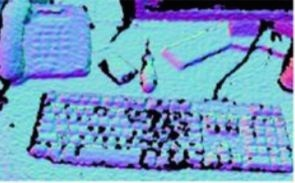
\includegraphics[width=0.4\columnwidth]{kinfu1.jpg}}
% 		\hfill
% 	\subfigure[Ground truth output]{%
% 		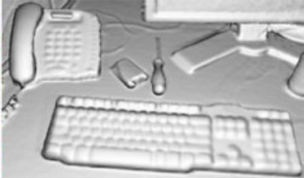
\includegraphics[width=0.4\columnwidth]{kinfu2.jpg}} \\
% 	\caption{Given a single RGBD image (\eg (a)), the aim is to predict the full, occupied volume of the scene (e.g. (b)).}
% \end{figure}

\subsubsection{Contributions}
\begin{itemize}
\item A scale-\emph{variant} mechanism for 6DOF hypothesis proposals, which is robust to local changes in geometrical appearance.
\item A classifier for verifying 6DOF hypotheses, trained on [synthetic/real] scenes
\item A probablistic method for combining together the per-voxel predictions of multiple hypotheses.
\end{itemize}

\subsubsection{Problem statement}

Setting out the problem mathematically, introducing some notation etc.

% What exactly do we mean by voxel occupancy?

% What is the scope of the work? 

% %%%%%%%%%%%%%%%%%%%%%%%%%%%%%%%%%%%%%%%%%%%%%%%%%%%%%%%%%%%%%%%%%%%%%%%%%%%%%%%%
\section{Related work}
% %%%%%%%%%%%%%%%%%%%%%%%%%%%%%%%%%%%%%%%%%%%%%%%%%%%%%%%%%%%%%%%%%%%%%%%%%%%%%%%%

% \paragraph{Axes of variation of related works}
% Using local information (\eg smoothing) $\leftrightarrow$ using global information (\eg patching from other images)

% Parametric models (Gaussian smoothing, CRFs) $\leftrightarrow$ non-parametric (patch-based)

% Care about semantic matching $\leftrightarrow$ Don't care about semantics


\paragraph{Nearest neighbours}
\cite{shen-tog-2012} use an assembly of parts from a CAD database to complete the unseen parts of a model given an RGBD image. 
While they demonstrate good results they assume they have semantic-specific models of the objects in the dataset.
Kim \ea \cite{kim-iccv-2013} use a CRF model over a voxel representation of a scene to simultaneously predict occupancy, visibility and semantical labelling of voxels from an RGBD image. 
For training, they use manually labelled top-down views of the scene. 
Their prediction of occupancy, however, is really just a Gaussian model. 
Final labellings found from graph cuts over the CRF. 
They make the observation that the observed values from a Kinect sensor can be very bad, and may need cleaning up.

Fouhey \ea \cite{fouhey-iccv-2013} use the NYU dataset of RGBD images to learn how to predict the normal orientations for each pixel of an input RGB image. 
In our case we are tackling a similar problem at a higher level --- we take RGBD as input, and aim to predict the full geometry of the scene.

\cite{guo-iccv-2013} use a single RGBD image to estimate the location and extent of the \emph{support surfaces} (\eg tabletops) in the scene. They do this by processing and analsing the geometry, before finally fitting shapes to the hypothesised support regions. They provide user-annotated 3D reconstructions of the full 3D space of the NYU dataset images, which could become useful for our work.


\paragraph{Mesh and image completion}
In the graphics community, there is a lot of work looking at the completion of missing and occluded parts of 3D meshes. 
For example, \cite{podolak-esgp-2005} fill holes in a mesh by enforcing watertightness across an octree structure, while \cite{schnabel-eurographics-2009} complete meshes by using primitives extracted from the areas of the scan without missing detail. 
A good overview of such mesh completion algorithms are given in \cite{ju-cst-2009}.

Image completion, such as \cite{hays-siggraph-2007}, typically has the aim of getting a good visually plausible output irrespective of the accuracy compared to ground truth. 
The results can be very impressive. 
Typically the image is completed by looking up possible completion regions in a large database of similar images.
RGBD datasets on the order of millions of images do not yet exist, so we need to take a different approach.

\paragraph{Super-resolution}
Similar to mesh completion is super-resolution, \eg \cite{macaodha-eccv-2012}. 
This, like our problem, is ill-posed and relies on the repeatability and predictability of the world in order to find suitable matches.

\cite{chang-tor-2007} complete a robot's map of an environment using parts of the already observed world to  `patch in' missing areas of the current map.

\paragraph{Symmetry}
Law and Aliaga \cite{law-cviu-2010} use symmetry to complete partial views. 
They are limited to only completing partial views; they rely on all objects being symmetrical; and they need user input.
Similarly, \cite{thrun-iccv-2005} and \cite{kroemer-humanoids-2012} use symmetry to complete models from a single depth view. 
They both demonstrate results on isolated objects, but not on more complex or cluttered scenes. 
The constraint of requiring axes of symmetry to both be present and accurately detected is a large limiting factor with these approaches.

\paragraph{Indoor room semantic prediction}
These works in general try to understand the semantic layout of a scene, \ie given an image infer what objects are in the scene and what their poses are.
\cite{nan-acm-2012, minkim-siggraphasia-2012}
This could be seen as finding one-to-many correspondences between models in a database and points in the scene.
In our work, by not restricting ourselves to trying to find semantic correspondences, we are able to model the shape of a far greater range of test scenes without making any assumptions about their semantic makeup.

\paragraph{Indoor room occupied space prediction}
\cite{hedau-cvpr-2012} seek to recover the free space in 2D images. They label ~500 images with box annotations, and aim to recover the bounding box layout of the scene in order to recover the free space.

In the vision community, most of the work is based around estimating the spatial layout of rooms from images.
For example \cite{bao-wacv-2014} use multiple images, before SfM and segmentation of the images. 
They then generate hypotheses of the layout. 
The hypotheses are chosen by evaluating their geometric cost, which is manually defined. 
They cite a lot of papers which do scene reasoning from a single image, but they argue that the problem is ill-posed (which it is). 

Using a single image, many people fit bounding boxes and try to estimate the layout using high-level info about gravity, typical scene arrangements etc. 
For example \cite{choi-cvpr-2013}.

\cite{lee-nips-2010} are another paper using a single image to estimate the layout of a room. 
Similarly, \cite{zhang-iccv-2013} infer the clutter and layout and support and segmentation and labelling from an RGBD image (using the NYU dataset).

\cite{hedau-cvpr-2012} seek to recover the free space in 2D images. 
They label ~500 images with box annotations, and aim to recover the bounding box layout of the scene in order to recover the free space. 
A big work in this area is that by \cite{gupta-cvpr-2011}, who estimate voxel occupation before fitting boxes.

Satkin \ea \cite{satkin-bmvc-2012} use 3D models to do scene understanding from a single image, and they demonstrate results on room scenes such as bedrooms and living rooms. 
A key interest for me is that they first propose hypotheses, before rendering them with OpenGL.
This then feeds into a hypothesis scorer which says if their ideas are any good. 
They form their proposals in an expensive way: they moving the cad model along the (x, y) scene axes, and render the model in every location, and in each of 4 rotation configurations!

\paragraph{6DOF object pose estimation}
Our work is closely related to the problem of estimating the 6DOF pose of a known database of objects in cluttered scenes, such as \cite{hinterstoisser-accv-2012, drost-3dimpvt-2012, rusu-iros-2010}. 
These work in many different ways; \cite{drost-3dimpvt-2012} aggregate pairwise features in a hash table to find the pose estimation --- they assume just one database model, which is assumed to be in the scene. \cite{rusu-iros-2010} first segment the scene, before looking up each segment in their training dataset.
All the methods nonetheless share the training step of rendering a 3D object from multiple angles.

All these methods so far assume that the item in the scene has the exact same geometry of the training instances.
\cite{cocias-cgvcv-2013} take an alternative approach, where they have a single primitive object for each class, which they fit to the scene and allow to deform to account for inter-class variation.

\paragraph{Robotics and path planning}
Voxels or 2D occupancy grids are often used in robotics for path planning, and for maintaining a map of the environment. These are typically deterministic approaches, \eg \cite{jetchev-icra-2010}. Sometimes a state model is used to model the states of voxels being occupied, unoccupied or unknown --- the voxel states are then updated as more information is gathered from sensors \cite{toussaint-techreport-2007}.

\cite{stentz-icra-1994} introduced D*, an algorithm similar to A* but for path planing in partially unknown environments. The world is in boxes, with arrows pointing to the direction which should be taken.
More recently, \cite{plagemann-iros-2008} used Gaussian processes to fill in missing data in terrain models of environments, effectively treating terrain mapping as a regression problem.

\paragraph{General motivation}
One key motivation is Shape Sharing \cite{kim-eccv-2012}, where silhouettes of objects are used to segment other objects from different classes.
 \cite{nan-acm-2012}.

Big issue with ground truth. Most papers don't have proper ground truth and therefore can only really do qualitative results, \eg \cite{all the papers...}.

\paragraph{To add to related work:}
\begin{itemize}
\item Box world --- predicting object locations and extents through bounding boxes.
\end{itemize}


% %%%%%%%%%%%%%%%%%%%%%%%%%%%%%%%%%%%%%%%%%%%%%%%%%%%%%%%%%%%%%%%%%%%%%%%%%%%%%%%%
\section{Approach}
% %%%%%%%%%%%%%%%%%%%%%%%%%%%%%%%%%%%%%%%%%%%%%%%%%%%%%%%%%%%%%%%%%%%%%%%%%%%%%%%%

% Overview of the method --- Figure \ref{fig:pipeline}.


% General motivation for method. Do not want to rely on having exact matches in training set. 
% Instead, want to find a collection of good matches in the training set which, when combined, will give a sensible prediction of the voxel occupancy.
% We take a RANSAC-style approach to finding basis shapes: first we \emph{propose} a set of candidate shapes which roughly match the scene, before we next \emph{re-weight} these candidates according to how well they match the scene geometry. 


% %%%%%%%%%%%%%%%%%%%%%%%%%%%%%%%%%%%%%%%%%%%%%%%%%%%%%%%%%%%%%%%%%%%%%%%%%%%%%%%%
\section{Methodology}
% %%%%%%%%%%%%%%%%%%%%%%%%%%%%%%%%%%%%%%%%%%%%%%%%%%%%%%%%%%%%%%%%%%%%%%%%%%%%%%%%

Requirements of the matching schema:
\begin{itemize}
\item Not looking to match the exact shapes --- instead want to match shapes that might only be somewhat similar
\item For this reason, want to be robust to local differences between the two regions, but capture the overall shape
\item Want the matching to be scale \emph{variant} --- should be able to match regions of the same shape regardless of their scale 
\item We therefore ultimately look for a 7DOF transformation
\end{itemize}

\paragraph{Scale variance}
We ensure we can match regions of the same shape but of different scales by rescaling each region by a scale factor $s$, where $s$ is the 95th percentile of the pairwise distances in the region. By using the 95th percentile instead of the maximum distance between pairs of points we become robust to outlying points.

\subsection{Predicting voxel occupancy}
The ultimate aim is to predict, for each voxel $v_k$ in the scene, the probably of the event $\occ_k$, \ie the probability that it is occupied or not. We therefore want $\prob(\occ_k | \rgbdimage)$ for each voxel.
$$
\prob(\occ_k | \rgbdimage) = \sum_{i,j} \prob(\occ_k|\basisshape_i)\prob(\basisshape_i|\imregion_j)\prob(\imregion_j|\rgbdimage)
$$

\begin{itemize}
\item $\prob(\occ_k|\basisshape_i)$ ---
This is $1$ if the voxel is inside the transformed basis shape mesh, and $0$ otherwise.
\item $\prob(\basisshape_i|\imregion_j)$ ---
This is the probability that basis shape $\basisshape_i$ is a correct match for region $\imregion_j$. We approximate this based on how well the region $\imregion_j$ matches the visible part of the $\basisshape_i$.
\item $\prob(\imregion_j|\rgbdimage)$ ---
This is the probability that the region of the image $\imregion_j$ is a correct segmentation of image $\rgbdimage$.
\end{itemize}

%%%%%%%%%%%%%%%%%%%%%%%%%%%%%%%%%%%%%%%%%%%%%%%%%%%%%%%%%%%%%%%%%%%%%%%%%%%%%%%%
\subsection{Pre-processing}
We assume we know the up direction of the scene. 
We find the largest plane with normals in this direction at the base of the scene, and segment out the areas above this.
We assume this plane is the tabletop or floor at the base of the image.


%%%%%%%%%%%%%%%%%%%%%%%%%%%%%%%%%%%%%%%%%%%%%%%%%%%%%%%%%%%%%%%%%%%%%%%%%%%%%%%%
\subsection{A soup of segments}

Our motivation for using a soup of segments together with class matching across class boundaries is like this. 
Imagine we had a chair in our test set. If in our training set we had a similar chair then we would like to use this, as it would hopefully be a good match. 
However, if we didn't have a chair in our training set then it is very unlikely that we would be able to find a suitable match. 
In this case, we would like to break up the chair into segments, each of which could have a similarly shaped object matched to it.


\begin{figure}
	\centering% 
	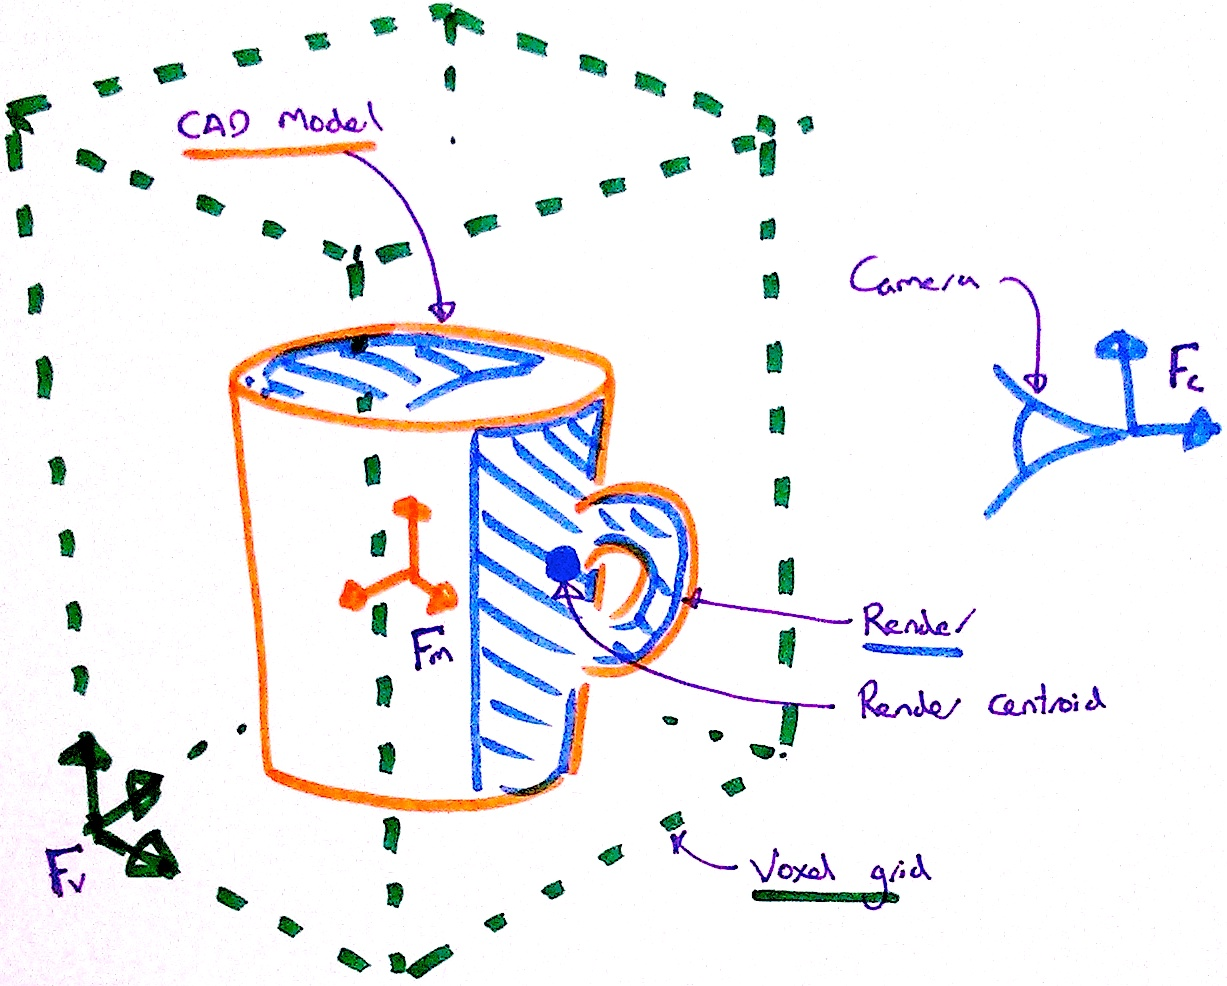
\includegraphics[width=1.0\linewidth]{voxel_coordinates}% 
	\figcaption{The interplay between the coordinate systems of the voxel grid, the camera the CAD model and the render for the synthetic rendered objects.}% 
	\label{fig:voxel_coordinates}% 
\end{figure}

% %%%%%%%%%%%%%%%%%%%%%%%%%%%%%%%%%%%%%%%%%%%%%%%%%%%%%%%%%%%%%%%%%%%%%%%%%%%%%%%%
% \subsection{Finding matches for each region}

% Find the $n$ nearest neighbours in $\chi^2$ distance space.

% %%%%%%%%%%%%%%%%%%%%%%%%%%%%%%%%%%%%%%%%%%%%%%%%%%%%%%%%%%%%%%%%%%%%%%%%%%%%%%%%
% \subsubsection{Features}

% Simple pairwise features very popular in RGBD image understanding, e.g. Drost, Shotton, Microsoft 7-scenes, FPFH, KinFu... 
% We use variants on the shape distribution \cite{osada-csma-2001} to form our FV. 
% Given a point cloud $\pcloud = \{\point_1, \hdots, \point_N\}$ with associated normals $\{\normal_1, \hdots, \normal_N\}$ we select random pairs of 
% $$
% \mathbf{f}_{i,j} = \left(|\point_i, \point_j|_2, \angle(\normal_i, \normal_j)\right),
% $$
% where $\angle(\normal_i,\normal_j)$ denotes the angle in radians between the normal vectors $\normal_i$ and $\normal_j$.
% We use the bag-of-words approach to aggregate the features for an entire region, into a feature vector. We use a dictionary with 75 words, formed using k-means.

% We don't necessarily have an exact match for each region or object in the database. We therefore allow for there to be 

% \subsection{Finding matches for each region}


% \subsection{Combining matches together}



% \subsection{For single object, single segmentation.}

% Image is $\rgbdimage$, event of occupancy is $o$. Basis shape is $\basisshape$.
% $$
% \prob(\occ | \rgbdimage) = \sum_i \prob(\occ | \basisshape) \prob(\basisshape | \rgbdimage)
% $$ 
% We know that $\prob(\occ|\basisshape)$ is just 1 within the shape, and 0 outside. 
% $\prob(\basisshape|\rgbdimage)$ is harder but could be based on some kind of heuristic based on number of inliers and how well the shape matches in etc.

% In particular:
% $$ 
% \sum_i \prob(\basisshape|\rgbdimage) = 1
% $$

% \subsection{For multiple segmentations.}

% Now we have to introduce the concept of segmentations. 
% The image $\rgbdimage$ will be segmented into a number of different regions $R$, where these regions may (but need not) overlap and the union of the regions need not cover the whole image.

% We can then perform the fitting as before, but this time on a per-region basis. The regions are then marginalised out:
% $$
% \prob(\occ | \rgbdimage) = \sum_{i,j} \prob(\occ|\basisshape)\prob(\basisshape|\imregion_j)\prob(\imregion_j|\rgbdimage)
% $$

% Similar to before,
% $$
% \sum_i \prob(\basisshape|\imregion) = 1
% $$

% However, there is no obligation for $\sum_j \prob(\imregion_j | \rgbdimage) = 1$, as the regions may be non-overlapping.

% The only thing left to compute is the probability of a specific region given the image, i.e. $\prob(\imregion_j|\rgbdimage)$. 

% $$
% \prob(\imregion_j | \rgbdimage) = \sum_{k} \prob(\imregion_j|S_k)\prob(S_k|\rgbdimage)
% $$
% $\prob(\imregion_j | S_k)$ is just the probability 


%%%%%%%%%%%%%%%%%%%%%%%%%%%%%%%%%%%%%%%%%%%%%%%%%%%%%%%%%%%%%%%%%%%%%%%%%%%%%%%%
\section{Experiments}
%%%%%%%%%%%%%%%%%%%%%%%%%%%%%%%%%%%%%%%%%%%%%%%%%%%%%%%%%%%%%%%%%%%%%%%%%%%%%%%%


\begin{figure}
	\centering% 
	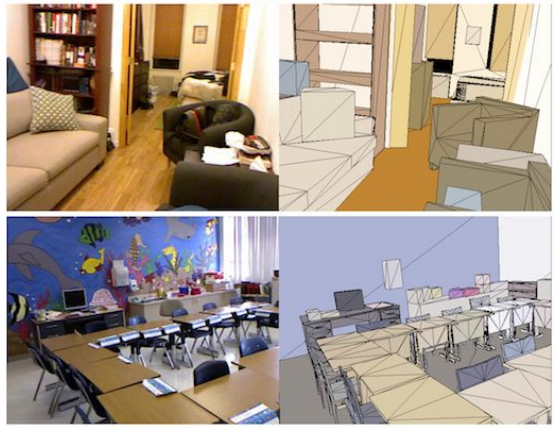
\includegraphics[width=1.0\columnwidth]{guo.png}% 
	\figcaption{Representation of objects in the NYU dataset, provided from \cite{guo-iccv-2013}. Not a perfect representation but perhaps reasonable to some extents.}% 
	\label{fig:guo_labels}% 
\end{figure}



\subsection{Database of CAD models}
Use the database from Fisher \ea \cite{fisher-siggraphasia-2012}.
1600 CAD models, each depth-rendered from 42 viewing angles using OpenGL.

\subsubsection{Potential test datasets}
\begin{itemize}
\item Create our own KinFu dataset
\item Kaparthy \ea --- would probably have to re-render their meshes. Also don't have the TSDF etc. Lots of problems
\item NYU dataset --- classic dataset. Potential ground truth labels from \cite{guo-iccv-2013} (figure \ref{fig:guo_labels}) or \cite{kim-iccv-2013}.
\item \cite{fisher-siggraphasia-2012}, use their synthetic scenes (great for a first pass!)
\end{itemize}


\begin{figure}
	\centering% 
	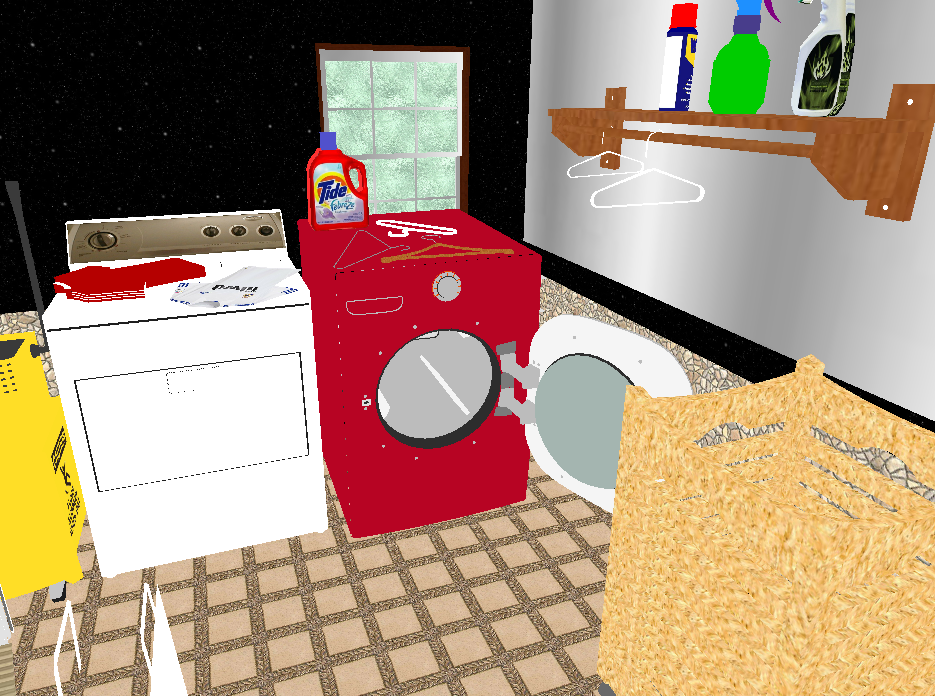
\includegraphics[width=1.0\columnwidth]{synth_scene.png}% 
	\figcaption{One of the user-created synthetic scenes from \cite{fisher-siggraphasia-2012}.}% 
	\label{fig:fisher_scene}% 
\end{figure}


%\bibliographystyle{plain}
\bibliographystyle{apalike}
\bibliography{bibtex/strings.bib,bibtex/main.bib,bibtex/crossrefs.bib}

%\end{multicols}
\end{document}